% Section 5: 3D reconstruction, camera model and calibration. Results: sections/eval_3d.tex (Section 8.3).
% Figures and numbers: writeup/make_camera_figures.py -> report/figures/camera/

\section{3D Reconstruction}
\label{sec:reconstruction}

The 3D position of the forceps tip is recovered from a single microscope image, using the tip and the shadow it
casts on the retina.

\subsection{Geometry}
\label{sec:reconstruction-geometry}

The eye is modelled as a sphere of radius $R = 12.05$\,mm, and the light as a point source $L$ at the tip of the
light pipe. A tip at $P$ casts its shadow $S$ where the ray from $L$ through $P$ meets the retina, so the tip lies on
the line from $L$ to $S$.

The far intersection of the shadow pixel's viewing ray with the eye sphere gives $S$; the tip is the point on
the line $LS$ closest to the viewing ray through the tip pixel. This is done for both jaws, and the reported tip is
their midpoint. Its height above the retina is $h = R - \lVert P \rVert$, with $P$ relative to the eye centre.

\subsection{Camera Model}
\label{sec:reconstruction-camera}

The first version of the pipeline used an \textbf{orthographic model}: parallel viewing rays, with one pixel-to-mm
scale taken from the visible eye circle (the circular field of view through the contact lens), whose edge was mapped to the eye's equator. Neither holds in the simulator.

The fitted effective camera centre (Section~\ref{sec:reconstruction-calibration}) lies only about 22\,mm from the
eye centre, so the image scale depends on depth: on the axis at the median tip height, a feature at the tip appears
about 21\,\% larger than on the retina behind it.
In addition, the edge of the visible circle is not the equator; the viewing
ray there meets the retina 9.6\,mm from the axis, not 12.05\,mm. Figure~\ref{fig:camera-geometry} shows the resulting error for
one tip.

The pipeline now uses a \textbf{perspective (pinhole) model}, in which the scale changes with depth by construction.
It is an effective model of the whole optical path, including contact lens and eye, not a physical camera position.

\begin{figure}[!htb]
  \centering
  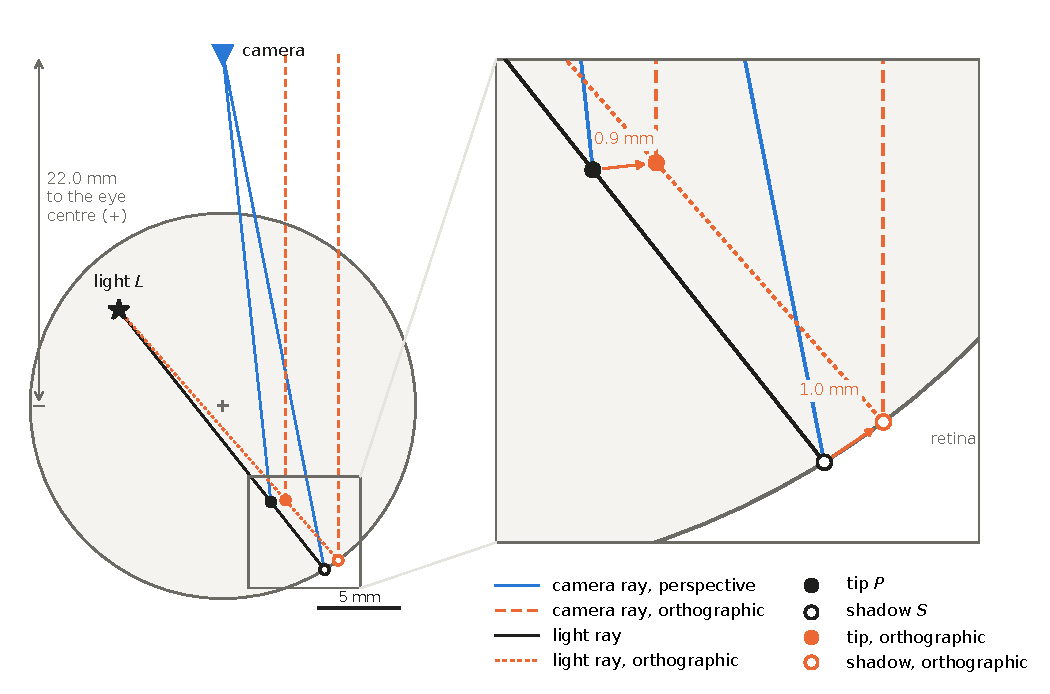
\includegraphics[width=0.85\linewidth]{figures/camera/geometry.pdf}
  \caption{Side cut through the eye, to scale; right: magnified. Blue: viewing rays of a pinhole at the fitted camera
    distance. Orange: the orthographic reading of the same two pixels; its tip is 0.9\,mm off and 0.4\,mm too low.}
  \label{fig:camera-geometry}
\end{figure}

\subsection{Calibration}
\label{sec:reconstruction-calibration}

The simulator exports with each video a trajectory log of the eye and instrument poses, which serves for calibration
and as ground truth (Section~\ref{sec:eval-3d}). Pairing logged and detected tip positions gives several thousand
3D--2D correspondences per recording, from which the camera projection and the time offset between video and log are fitted (median reprojection error below 0.5\,px).

The trocars are fitted from the logged instrument axes; $L$ is placed at the light pipe's median logged insertion depth and aim.

Zoom and contact-lens distance were kept fixed, and the two recordings of one session give nearly the same camera (focal
length within 0.2\,\%, centre within 0.2\,mm). The eye's rotation about the viewing axis can differ by several degrees between sessions and is measured once per
session from the trocar positions in the image.
